\documentclass{beamer}
\usepackage[utf8]{inputenc}
\usepackage{caption}
\usepackage{subcaption}
\usepackage{amsmath}
\usepackage{tikz}

\title{Math Camp Day 1}
\author{Ben Adenbaum, Juanita Duque-Rosero, Ryan Maguire, Kameron McCombs}
\date{August 2021}
\usenavigationsymbolstemplate{}
\setbeamertemplate{footline}[frame number]
\begin{document}
    \maketitle
    \begin{frame}{Outline}
        \begin{itemize}
            \item The game hex.
            \item Applying hex to topology.
            \item Coffee.
        \end{itemize}
    \end{frame}
    \begin{frame}{Hex}
        Hex is a combinatorial game, it is W-L-D, and it is NOT
        impartial (try to explain why to yourself). Two players take turns coloring
        hexagons red and blue. The first to connect end-to-end with a single
        color wins.
        \begin{figure}
            \centering
            \includegraphics[scale=1.5]{hex_11x11.eps}
            \caption{Hex}
            \label{fig:hex_11x11}
        \end{figure}
    \end{frame}
    \begin{frame}{Hex}
        Go play!
    \end{frame}
    \begin{frame}{Hex}
        What is a draw in hex? Can you show a draw in impossible in this game?
        \begin{figure}
            \centering
            \includegraphics{hex_2x2.eps}
            \caption{Simple Hex}
            \label{fig:hex_2x2}
        \end{figure}
    \end{frame}
    \begin{frame}{Hex}
        How about this game?
        \begin{figure}
            \centering
            \includegraphics{hex_3x3.eps}
            \caption{Not-as-simple Hex}
            \label{fig:hex_3x3}
        \end{figure}
    \end{frame}
    \begin{frame}{Hex}
        And lastly, how about this?
        \begin{figure}
            \centering
            \includegraphics{hex_5x5.eps}
            \caption{Sligthly harder Hex}
            \label{fig:hex_5x5}
        \end{figure}
    \end{frame}
    \begin{frame}{Hex}
        Now let's play \textit{Anti-Hex}. The first player to
        connect end to end \textit{loses}. In other words, the first
        player to win in normal hex is the player that loses in
        anti-hex.
        \begin{figure}
            \centering
            \includegraphics{hex_7x7.eps}
            \caption{7x7 Hex}
            \label{fig:hex_7x7}
        \end{figure}
    \end{frame}
    \begin{frame}{Hex}
        Is it possible to draw hex? We've seen in the 2x2, 3x3, and 5x5 case that this is impossible
        since there are only so many moves to play. In the 7x7 case we tried our best \textit{not} to win,
        but someone ended up winning. How about the 11x11 case? Well, first a question:
        \begin{center}
            Are there more 11x11 hex games, or more chess games?
        \end{center}
    \end{frame}
    \begin{frame}{Hex}
        There are about 100 trillion \textit{times} more 11x11 hex games than chess games. That is, for every
        1 chess game, there are about 100 trillion 11x11 hex games. So trying to solve this brute force is
        out of the question. In comes the connection between \textit{game theory} and \textit{topology}.
    \end{frame}
    \begin{frame}{Coffee}
        Image you have a coffee cup that needs stirring. You also have incredibly sharp eyes and
        can keep track of every single molecule. After you've done some stirring, you ask the
        following question:
        \begin{center}
            Is there a molecule that didn't move?
        \end{center}
        What do you think?
    \end{frame}
    \begin{frame}{Coffee}
        Let's try the \textit{1-dimensional} analogue. We have a bunch of
        particles in a line. We move the particles along the line in a
        \textit{continuous} motion. Is there a particle that didn't move?
        The benefit of the 1D case is we can draw a nice convincing picture.
    \end{frame}
    \begin{frame}{Coffee}
        The $x$ axis is our starting line. For every point in the $x$ axis, we must
        pick a point in the $y$ axis, this is where that particle went. Since it is
        \textit{continuous}, in the end we have a continuous curve that fits inside
        a box. A particle that didn't move would lie on the line $y=x$. So we ask,
        is it possible to draw a line from the blue on the left to the blue on the
        right without crossing the diagonal?
        \begin{figure}
            \centering
            \includegraphics[scale=0.9]{brouer_fixed_point_1d.eps}
            \caption{1D Coffee}
            \label{fig:brouer_fixed_point_1d}
        \end{figure}
    \end{frame}
    \begin{frame}{Coffee}
        The answer is pretty intuitively \textit{no}. The coffee theorem
        is when we are asking about the unit disk instead of a line.
        Brouwer's Fixed Point Theorem says there is always a coffee molecule
        that didn't move. This hold for all dimensions, so if you have
        24 dimensional coffee, the result is still true.
    \end{frame}
    \begin{frame}{Coffee}
        To avoid confusion, you can't have a bizarre coffee cup. It has
        to be a cylindrical cup. No torus cups, and no infinitely long cups.
        If you had such a cup, the result is false.
        \begin{figure}
            \centering
            \rotatebox{90}{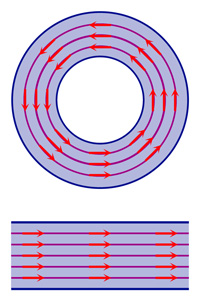
\includegraphics[scale=0.7]{brouwer_bad.jpg}}
            \caption{Brouwer Doesn't Apply}
            \label{fig:brouwer_bad}
        \end{figure}
    \end{frame}
    \begin{frame}{Hex}
        How does this relate to hex? Brouwer's fixed point theorem allows us to
        prove the following.
        \begin{theorem}
            It is impossible to draw a game of hex.
        \end{theorem}
        The proof is a little involved, but there's something even more remarkable.
    \end{frame}
    \begin{frame}{Hex}
        \begin{theorem}
            If the game of Hex is impossible to draw, then
            Brouwer's fixed point theorem is true.
        \end{theorem}
        That is, we can use a result about game theory to prove one of
        the most important theorems of topology! Historically, it went the
        other way around. Brouwer's theorem was proved in the 1910's where as this hex
        theorem came about in the 1940's, but it's still incredible!
    \end{frame}
    \begin{frame}{Hex}
        One final note, the only mathematician to ever receive the Nobel prize%
        \footnote{John Nash won the economics Nobel prize in 1994. There is no Nobel prize in mathematics.}
        \footnote{Other mathematicians have won Nobel prizes, but for other works, usually physics or philosophy.}
        won it for work related to connecting game theory and topology.
    \end{frame}
\end{document}